\documentclass[letterpaper,article,11pt,oneside]{memoir}
\usepackage{etoolbox}	% enables boolean variables and logic
%----------------------------------------------------------------------------
% Define Boolean Variables
%----------------------------------------------------------------------------
\newbool{mtpro2font}
\newbool{beramono}
\newbool{boldtitle}
\newbool{subtitledisplayed}
\newbool{sectionnumbers}
\newbool{authdatedisplayed}
%----------------------------------------------------------------------------
% Set Document Formatting Choices
%----------------------------------------------------------------------------
\setbool{mtpro2font}{false}
\setbool{beramono}{true}		% monospaced font; courier if false
\setbool{boldtitle}{true}
\setbool{subtitledisplayed}{true}
\setbool{sectionnumbers}{false}	% number section headings or not
\setbool{authdatedisplayed}{true}
\newcommand{\foliosize}{\normalsize}
\newcommand{\headersize}{\small}
%----------------------------------------------------------------------------
% Font Choices
%----------------------------------------------------------------------------
\usepackage[T1]{fontenc}			% use T1 font encoding
\usepackage[scaled=0.92]{helvet}	% set Helvetica as the sans-serif font
\ifbool{mtpro2font}                 % set font based on boolean
	{
		\usepackage{times}%         % set times as text font
		\usepackage[subscriptcorrection,slantedGreek,nofontinfo]{mtpro2} % set math time pro 2 as the math font
	}
	{
		\usepackage[sc]{mathpazo}%  % set Palatino math and body font
	 	\linespread{1.05}%          % increase line spacing for Palatino
	 }
\ifbool{beramono}
	{
		\usepackage[scaled=0.90]{beramono}  % beramono as monospaced font
	}
	{
		\usepackage{courier}               	% courier as monospaced font
	}
%----------------------------------------------------------------------------
% Load Packages
%----------------------------------------------------------------------------
\usepackage{lipsum}     % produces blocks of lipsum text
\usepackage{titlesec}   % allows modification of heading formats
\usepackage{microtype}	% allows adjustment of letter spacing
\usepackage{layout}
\usepackage{graphicx}
%----------------------------------------------------------------------------
% Set Page Dimensions
%----------------------------------------------------------------------------
%\settypeblocksize{541pt}{360pt}{*} % 30 pica measure
\settypeblocksize{541pt}{336pt}{*} % 28 pica measure
%----------------------------------------------------------------------------
% Define Document Title, Author, and Date
%----------------------------------------------------------------------------
\newcommand{\doctitle}{Single Sided Report for Physical Chemistry}
\newcommand{\docauthor}{Dale J. Brugh}
\newcommand{\docdate}{\today}
% Create Lowercase Version of Document Title
% This is for use in headers
\DeclareRobustCommand*\DefLowercaseDoctitle{% 
  \gdef\LowercaseDoctitle
 }
\MakeLowercase{\DefLowercaseDoctitle{\doctitle}} 
% Set Title, Author, Date
\title{\doctitle}
\author{\docauthor}
\date{\docdate}
%----------------------------------------------------------------------------
% Format Section Headings
%----------------------------------------------------------------------------
\counterwithout{section}{chapter}
%\makeheadstyles{bringhurst}{%
%\renewcommand*{\subsecheadstyle}{\normalfont\large\itshape}
%}
%\headstyles{bringhurst}
% Turn section numbers on or off depending on value of sectionnumbers
\ifbool{sectionnumbers}
{
    \setsecnumdepth{subsection}  % displays section numbers	
}
{
    \setsecnumdepth{part}  % removes section numbers		
}

%----------------------------------------------------------------------------
% Small Caps Page Style
%----------------------------------------------------------------------------
% This page style is inspired by Tufte's books. It places the 
% section title and folio in the right header slot on recto pages and 
% in the left header slot on verso pages. 
%
\nouppercaseheads
\makepagestyle{smallcaps}
\newlength{\newheaderwidth}
\setlength{\newheaderwidth}{\textwidth}
\makerunningwidth{smallcaps}{\newheaderwidth}
\clearmark{section}
% Assign section name without number to rightmark
\createmark{section}{right}{nonumber}{}{}
% Assign chapter name without number to leftmark
%\createmark{title}{left}{nonumber}{}{}

\makeoddhead{smallcaps}{}{}{\textls*[50]{\headersize\scshape\rightmark}~~~~~~\foliosize\thepage}
\makeevenhead{smallcaps}{\foliosize\thepage~~~~~~\textls*[50]{\headersize\scshape\rightmark}}{}{}

\pagestyle{smallcaps}
%----------------------------------------------------------------------------
% Document Begins
%----------------------------------------------------------------------------
\begin{document}
%\layout
\maketitle
\thispagestyle{empty}

\noindent This is a single-column report built on the \LaTeX\ memoir class. It is best typeset as a one-sided document. This document template should be used when writing reports in physical chemistry at Ohio Wesleyan University. 

\section{Abstract}
Some reports will require an abstract. You do not need to apply special formatting to the abstract. Just make it another section in your report. 

\section{Equations}
The three dimensional Schr\"odinger equation in Cartesian coordinates is given by
\begin{equation}\label{eq-schrodinger}
-\frac{\hbar^2}{2m}\left[\frac{\partial^2}{\partial x^2} + \frac{\partial^2}{\partial y^2} + \frac{\partial^2}{\partial z^2}\right]\psi(x,y,z) = E \psi(x,y,z)
\end{equation}
where $m$ is the mass of the particle and $E$ is the total energy of the particle. Note that Equation~\ref{eq-schrodinger} is an equation in display mode while $m$ and $E$ are in what is called inline math mode. This also illustrates how to reference equations. 

\section{Tables}
If you want to include a table in a report, this is how you should do it. Rows in a table end with a double backslash. Cells are separated with an amperstand. The material in Table~\ref{tab-illustration} is just randome stuff that has no meaning. 
\begin{table}[h]
\caption{This is the first table.}
\begin{tabular}{lcr}
\hline\hline
Cell 1 & Cell 2 & Cell 3 \\
Cell 4 & Cell 5 & Cell 6 \\
Cell 7 & Cell 8 & Cell 9 \\
\hline\hline
\end{tabular}
\label{tab-illustration}
\end{table}
You should not try to manually move a table around in your report. Instead, you should insert the table where it logically belongs and then allow \LaTeX\ to position it. \LaTeX\ will almost always make better choices than you will make. 

If, however, you really feel like you must adjust the position of a table, you can change the h to b or t after beginning a table. 

\section{Figures}
Figures should be included in this way. Always refer to figures and tables by number. If you want to refer to Figure~\ref{fig-boltzmann} you do so with the \LaTeX\ reference command. 
\begin{figure}[h]
\caption{Photograph of Boltzmann taken from Wikipedia.}
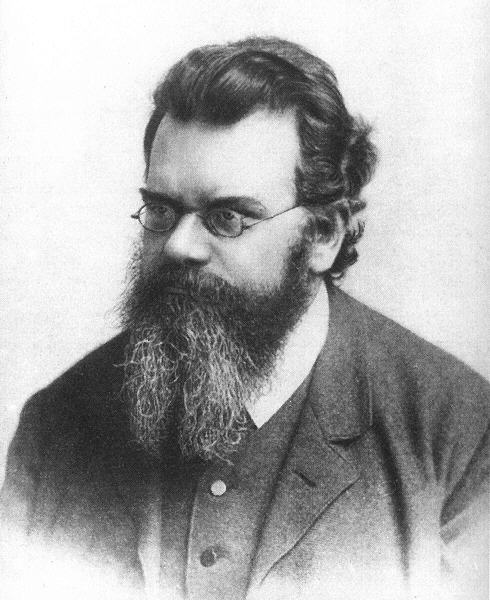
\includegraphics[width=1.5in]{figs/Boltzmann2.jpg}
\label{fig-boltzmann}
\end{figure}
%----------------------------------------------------------------------------
\end{document}